\documentclass[a4paper,10pt,ceqn,dvipsnames,twoside,openright]{memoir}  	% Openright aabner kapitler paa hoejresider (openany begge)


%%%% PACKAGES %%%%
% ¤¤ Oversaettelse og tegnsaetning ¤¤ %
\usepackage[utf8]{inputenc}					% Input-indkodning af tegnsaet (UTF8)
\usepackage[english]{babel}					% Dokumentets sprog
\usepackage[OT1]{fontenc}					% Output-indkodning af tegnsaet (T1)
\usepackage{ragged2e,anyfontsize}			% Justering af elementer
\usepackage{mfirstuc}

% ¤¤ Packages for the solar panel figure ¤¤ %
\usepackage{xcolor}
\usepackage[american,cuteinductors,smartlabels]{circuitikz}
\usepackage{siunitx}
\usetikzlibrary{calc}
\usetikzlibrary{patterns}
\ctikzset{bipoles/thickness=1}
\ctikzset{bipoles/length=0.8cm}
\ctikzset{bipoles/diode/height=.375}
\ctikzset{bipoles/diode/width=.3}
\ctikzset{tripoles/thyristor/height=.8}
\ctikzset{tripoles/thyristor/width=1}
\ctikzset{bipoles/vsourceam/height/.initial=.7}
\ctikzset{bipoles/vsourceam/width/.initial=.7}
\tikzstyle{every node}=[font=\small]
\tikzstyle{every path}=[line width=0.8pt,line cap=round,line join=round]

\definecolor{AleeRed}{rgb}{0.5,0,0}
\definecolor{gray75}{gray}{0.75}
\usepackage{graphicx}
\usepackage{adjustbox}
\usepackage{epstopdf}

\usepackage{subcaption}

%Roman letters
\ExplSyntaxOn
\NewDocumentCommand{\RN}{m}
 {
  \textup{ \int_to_Roman:n { #1 } }
 }
\ExplSyntaxOff

																			
% ¤¤ Figurer og tabeller (floats) ¤¤ %
\usepackage{graphicx} 						% Haandtering af eksterne billeder (JPG, PNG, EPS, PDF)
\usepackage{multirow}                		% Fletning af raekker og kolonner (\multicolumn og \multirow)
\usepackage{multicol}         	        	% Muliggoer output i spalter
\usepackage{rotating}						% Rotation af tekst med \begin{sideways}...\end{sideways}
\usepackage{colortbl} 						% Farver i tabeller (fx \columncolor og \rowcolor)

\usepackage{flafter}						% Soerger for at floats ikke optraeder i teksten foer deres reference
\let\newfloat\relax 						% Justering mellem float-pakken og memoir
\usepackage{float}							% Muliggoer eksakt placering af floats, f.eks. \begin{figure}[H]
\newcommand{\HRule}{\rule{\linewidth}{0.5mm}}
\usepackage{pdflscape}	 					% Giver mulighed for landacape mode
\usepackage{longtable}						% Giver mulighed for talber over flere side
%\usepackage{subcaption}
\usepackage{capt-of}

 %\usepackage{nccmath}

% ¤¤ Matematik mm. ¤¤
\usepackage{amsmath}						% Avancerede matematik-udvidelser
\usepackage{blkarray}
\usepackage{amssymb}						% Avancerede matematik-udvidelser
\usepackage{stmaryrd}						% Avancerede matematik-udvidelser
\usepackage{amsthm}							% Avancerede matematik-udvidelser
\usepackage{textcomp}                 		% Symbol-udvidelser (f.eks. promille-tegn med \textperthousand )
\usepackage{mathtools}
\usepackage{lmodern,bm}                
\usepackage[T1]{sansmath} 
\SetMathAlphabet{\mathsfbf}{sans}{\sansmathencoding}{\sfdefault}{bx}{sl}
\usepackage{etoolbox}
\AtBeginEnvironment{sansmath}{\let\bm\mathsfbf}{}{}
\DeclareRobustCommand{\ttfamily}{\fontencoding{T1}\fontfamily{lmtt}\selectfont}

\expandafter\def\expandafter\normalsize\expandafter{%
    \normalsize
    \setlength\abovedisplayskip{10pt}
    \setlength\belowdisplayskip{10pt}
    \setlength\abovedisplayshortskip{10pt}
    \setlength\belowdisplayshortskip{10pt}
}

\usepackage{gensymb}

% ¤¤ Kode indsat i rapport ¤¤ %
\usepackage{listings}						% Placer kildekode i dokumentet med \begin{lstlisting}...\end{lstlisting}



\usetikzlibrary{decorations.pathmorphing}
%\usepackage[detect-all]{siunitx}

\tikzset{
   ragged border/.style={ decoration={random steps, segment length=1mm, amplitude=0.5mm},
           decorate,
   }
}

  \usetikzlibrary{arrows}
\usepackage{array}
\newcolumntype{P}[1]{>{\centering\arraybackslash}p{#1}}
\newcolumntype{M}[1]{>{\centering\arraybackslash}m{#1}}


% ¤¤ Matematik funktioner ¤¤				% Sikre alle funktioner står med ordinær skriftype
	\newcommand{\e}{\text{e}}
	\newcommand{\dB}{\text{dB}}	
	\newcommand{\I}{\text{I}}	
	\newcommand{\V}{\text{V}}
	\newcommand{\A}{\text{A}}
	\newcommand{\W}{\text{W}}
	\newcommand{\F}{\text{F}}
	\renewcommand{\S}{\text{S}}	
	\newcommand{\rms}{\text{rms}}
	\newcommand{\m}{\text{m}}
	\newcommand{\n}{\text{n}}
	\newcommand{\p}{\text{p}}
	\newcommand{\f}{\text{f}}
	\renewcommand{\k}{\text{k}}
	\newcommand{\M}{\text{M}}
	\newcommand{\G}{\text{G}}
	\newcommand{\C}{\text{C}}
	\renewcommand{\c}{\text{c}}
	\newcommand{\T}{\text{T}}
	\newcommand{\km}{\text{km}}
	\newcommand{\h}{\text{h}}		
	\newcommand{\s}{\text{s}}
	\newcommand{\cm}{\text{cm}}
	\newcommand{\ms}{\text{ms}}


% ¤¤ Opsætning af enheder ¤¤ % 
	\newcommand{\unit}[1]{\hfill\left[\mathrm{ #1}\right]} 	% Skriv \enhed{"din enhed"} og dem bliver rykket til højre


% ¤¤ Referencer og kilder ¤¤ %
			
\usepackage[square, numbers, comma, sort&compress]{natbib}			
\bibliographystyle{ieeetr}
% Udseende af litteraturlisten.

% ¤¤ Textlable setup ¤¤ % 
\makeatletter
\newcommand*{\textlabel}[2]{				% Gør \textlabel mulig
  \edef\@currentlabel{#1}					% Set target label
  \phantomsection							% Correct hyper reference link
  #1\label{#2}}								% Print and store label

% ¤¤ Misc. ¤¤ %
\usepackage{lipsum}							% Dummy text \lipsum[..]
\usepackage[shortlabels]{enumitem}			% Muliggoer enkelt konfiguration af lister
\usepackage{pdfpages}						% Goer det muligt at inkludere pdf-dokumenter med kommandoen \includepdf[pages={x-y}]{fil.pdf}	
\pdfoptionpdfminorversion=6					% Muliggoer inkludering af pdf dokumenter, af version 1.6 og hoejere
\pretolerance=2500 							% Justering af afstand mellem ord (hoejt tal, mindre orddeling og mere luft mellem ord)

% Kommentarer og rettelser med \fxnote. Med 'final' i stedet for 'draft' udloeser hver note en error i den faerdige rapport.
\usepackage[footnote,draft,danish,silent,nomargin]{fixme}
\renewcommand{\thefootnote}{\arabic{footnote}}

%%%% CUSTOM SETTINGS %%%%

% ¤¤ Marginer ¤¤ %
\setlrmarginsandblock{3cm}{3.0cm}{*}		% \setlrmarginsandblock{Indbinding}{Kant}{Ratio}
\setulmarginsandblock{3.2cm}{3.0cm}{*}		% \setulmarginsandblock{Top}{Bund}{Ratio}
\checkandfixthelayout 						% Oversaetter vaerdier til brug for andre pakker

%	¤¤ Paragraph formatting ¤¤ %
\setlength{\parindent}{0mm}           		% Stoerrelse af indryk
\setlength{\parskip}{3mm}          			% Afstand mellem afsnit ved brug af double Enter
\linespread{0.95}								% Linie afstand

% ¤¤ Table of contents ¤¤ %
\setsecnumdepth{subsubsection}		 			% Dybden af nummerede overkrifter (part/chapter/section/subsection)
\maxsecnumdepth{subsubsection}				% Document class boundary for numbering depth
\settocdepth{subsubsection} 					% Dybden af indholdsfortegnelsen

% ¤¤ Lister ¤¤ %
\setlist{
  topsep=0pt,								% Vertikal afstand mellem tekst og listen
  itemsep=-1ex,								% Vertikal afstand mellem items
} 

% ¤¤ Visuelle referencer ¤¤ %
\usepackage[colorlinks]{hyperref}			% Danner klikbare referencer (hyperlinks) i dokumentet.
\hypersetup{colorlinks = true,				% Opsaetning af farvede hyperlinks (interne links, citeringer og URL)
    linkcolor = black,
    citecolor = blue,
    urlcolor = blue
}

% ¤¤ Opsaetning af figur- og tabeltekst ¤¤ %
\captionnamefont{\small\bfseries\itshape}	% Opsaetning af tekstdelen ('Figur' eller 'Tabel')
\captiontitlefont{\small}					% Opsaetning af nummerering
\captiondelim{. }							% Seperator mellem nummerering og figurtekst
\hangcaption								% Venstrejusterer flere-liniers figurtekst under hinanden
\setlength{\belowcaptionskip}{0pt}			% Afstand under figurteksten



\let\oldequation=\equation
\let\endoldequation=\endequation
\renewenvironment{equation}{\vspace{-6mm}\begin{oldequation}}{\end{oldequation}\vspace{-6mm}}

% ¤¤ Navngivning ¤¤ %
\addto\captionsdanish{
	\renewcommand\appendixname{Appendix}
	\renewcommand\contentsname{Table of contest}	
	\renewcommand\appendixpagename{Appendix}
	\renewcommand\appendixtocname{Appendix}
	\renewcommand\cftchaptername{\chaptername~}				% Skriver "Kapitel" foran kapitlerne i indholdsfortegnelsen
	\renewcommand\cftappendixname{\appendixname~}			% Skriver "Appendix" foran appendiks i indholdsfortegnelsen
}

% ¤¤ Kapiteludssende ¤¤ %
\definecolor{numbercolor}{gray}{0.7}		% Definerer en farve til brug til kapiteludseende
\newif\ifchapternonum

\makechapterstyle{AlexanderGrebenkov}{%
\renewcommand{\chapterheadstart}{\vspace*{0cm}\hrule height 1.1pt\vspace{0.2cm}\medskip}
\renewcommand{\chapnamefont}{\normalfont\huge\bfseries}
\renewcommand{\chapnumfont}{\normalfont\huge\bfseries}
\renewcommand{\chaptitlefont}{\normalfont\huge\bfseries}
\renewcommand{\printchaptername}{}
\renewcommand{\chapternamenum}{ }
\renewcommand{\printchapternum}{\chapnumfont \thechapter}
\renewcommand{\afterchapternum}{. }
\renewcommand{\afterchaptertitle}{\par\nobreak\medskip\vspace{0.2cm}\hrule height 1.1pt\vspace{0.4cm}}
}
\chapterstyle{AlexanderGrebenkov}

% ¤¤ Header ¤¤ % 

\makepagestyle{AAU}							% Definerer sidehoved og sidefod udseende frem til ...
\makepsmarks{AAU}{%
	\createmark{chapter}{left}{shownumber}{}{. \ }
	\createmark{section}{right}{shownumber}{}{. \ }
	\createplainmark{toc}{both}{\contentsname}
	\createplainmark{lof}{both}{\listfigurename}
	\createplainmark{lot}{both}{\listtablename}
	\createplainmark{bib}{both}{\bibname}
	\createplainmark{index}{both}{\indexname}
	\createplainmark{glossary}{both}{\glossaryname}
}
\nouppercaseheads											% Ingen Caps oenskes



\makeevenhead{AAU}{}{}{\leftmark}					    % Definerer lige siders sidehoved (\makeevenhead{Navn}{Venstre}{Center}{Hoejre})
\makeoddhead{AAU}{\rightmark}{}{Aalborg University}			% Definerer ulige siders sidehoved (\makeoddhead{Navn}{Venstre}{Center}{Hoejre})
\makeheadrule{AAU}{\textwidth}{0.5pt}						% Adds a line under the header content

\makefootrule{AAU}{\textwidth}{0.5pt}{0.5mm}					% Adds a line below the footer's content

\copypagestyle{AAUchap}{AAU}								% Page header for chapter pages is defined as standard pages but with blank header
\makeoddhead{AAUchap}{}{}{}
\makeevenhead{AAUchap}{}{}{}
\makeheadrule{AAUchap}{\textwidth}{0pt}
\aliaspagestyle{chapter}{AAUchap}							% Den ny style vaelges til at gaelde for chapters
															% ... her
															
\pagestyle{AAU}												% Valg af sidehoved og sidefod


%%%% CUSTOM COMMANDS %%%%

% ¤¤ Specielle tegn ¤¤ %
\newcommand{\decC}{^{\circ}\text{C}}
\newcommand{\dec}{^{\circ}}


%%%% ORDDELING %%%%

\hyphenation{}

%%%% GlOSSARIES %%%%
%\usepackage[toc,nowarn]{glossaries}
%\makeglossaries
%
%% \newacronym{label}{short name}{long name}







%% \newglossaryentry{label}{name={the real name}, description={robots are the better humans}}

%\makeatletter\@openrightfalse\makeatother


%%%% COOL EXTRA FEATURES %%%%%
\usepackage{lastpage}
\usepackage{todonotes}
\newcommand{\todotom}[1]{\todo[color=red!40, author=Tom]{#1}}
\graphicspath{{./rapport/billeder/}}
\newcommand{\todoque}[1]{\todo[color=red, author=Question:]{#1}}
\graphicspath{{./rapport/billeder/}}
\usepackage{epstopdf}
%dashed line in matrix
\usepackage{arydshln}

\usepackage{pdflscape}
\usepackage{bbm}
\usepackage{dsfont}




%%%% WARNING HACKS %%%%
\hfuzz=\maxdimen
\tolerance=100000
\hbadness=\maxdimen
\vbadness=\maxdimen
\vfuzz=\maxdimen


%%%% NICE LOOKING REFERENCE %%%%
\newcommand{\itref}[1]{\textit{\ref{#1}}}
\newcommand{\chapref}[1]{Chapter \textit{\ref{#1}: \nameref{#1}}}
\newcommand{\secref}[1]{Section \textit{\ref{#1}: \nameref{#1}}}
\newcommand{\figref}[1]{\emph{Figure \ref{#1}}}
\newcommand{\appref}[1]{\emph{Appendix: \ref{#1}}}
\newcommand{\tabref}[1]{\emph{Table: \ref{#1}}}
\newcommand{\coderef}[1]{\emph{Listings: \ref{#1}}}
\renewcommand{\eqref}[1]{\emph{Equation: (\ref{#1})}}


%%%% TIKZ MAGIC %%%%
\usepackage{schemabloc}
\usetikzlibrary{circuits}
\usepackage{tikz}
\usetikzlibrary{shapes,arrows}
\usepackage{pgfplots}
\usetikzlibrary{plotmarks}
\usetikzlibrary{fit}
\pgfplotsset{compat=newest}
\pgfplotsset{filter discard warning=false}
%\usepackage[americanresistors,americaninductors,american voltages]{circuitikz}
\usetikzlibrary{calc}
\usetikzlibrary{patterns}
\ctikzset{bipoles/thickness=1}
\ctikzset{bipoles/length=0.8cm}
\ctikzset{bipoles/diode/height=.375}
\ctikzset{bipoles/diode/width=.3}
\ctikzset{tripoles/thyristor/height=.8}
\ctikzset{tripoles/thyristor/width=1}
\ctikzset{bipoles/vsourceam/height/.initial=.7}
\ctikzset{bipoles/vsourceam/width/.initial=.7}
\tikzstyle{every node}=[font=\small]
\tikzstyle{every path}=[line width=0.8pt,line cap=round,line join=round]
\definecolor{AleeRed}{rgb}{0.5,0,0}
\newcommand\addvmargin[1]{
  \node[fit=(current bounding box),inner ysep=#1,inner xsep=0]{};
}
\usetikzlibrary{positioning}

% \usetikzlibrary{external}
% \tikzexternalize[prefix=tikz/]

%%%% CDO FIX %%%%
\usepackage{silence}
\WarningsOff[pgfplots]
\WarningFilter{latex}{Marginpar on page}
\WarningFilter{memoir}{You are using the caption package with the memoir class}
\WarningsOff[latex]
\WarningFilter{LaTeX Font Warning:}{Font shape `U/stmry/b/n' undefined(Font)              using `U/stmry/m/n' instead on input line 5.}



 \renewcommand{\familydefault}{\rmdefault}


\usetikzlibrary{shapes,positioning,matrix}
\usetikzlibrary{decorations.pathreplacing}

\newcommand{\noop}[1]{} 

\begin{document}
\frontmatter
\makeevenfoot{AAU}{\thepage}{}{}
\makeoddfoot{AAU}{}{}{\thepage}

\pagenumbering{gobble}
\section{Identification notes}

\subsection{System equations}

The output $\bar{p}_{\mathcal{K}}$ is given by \eqref{eq1}, which is a static equation

\begin{equation}
  \label{eq1}
  \bar{p}_{\mathcal{K}} = K^T \bar{H}^{-T}_{\mathcal{T}}f_{\mathcal{T}}(A_2 q_\mathcal{C} + A_3 K \bar{d}_{\mathcal{K}} - A_3 D v_{\mathcal{D}} \sigma) - \underbrace{K^T\bar{H}^{-T}_{\mathcal{T}}\hat{H}^{T}_{\mathcal{T}} (\hat{p} + \hat{h}) - K^T\bar{h}}_{\text{Linear term}} .
\end{equation}

We consider it as an input-output model where the inputs:

 \begin{minipage}[t]{0.2\textwidth}
\hspace*{6mm} $K^T\bar{h} = \bar{h}_{\mathcal{K}} $ \\
\hspace*{6mm} $\hat{p}$  \\
\hspace*{6mm} $\hat{h}$ \\
\hspace*{6mm} $\sigma$ \\
\hspace*{6mm} $\bar{d}_{\mathcal{K}}$ \\
\hspace*{6mm} $q_\mathcal{C}$
\end{minipage}
\begin{minipage}[t]{0.58\textwidth}
%\vspace*{2mm}
is the elevation of inlets ,\\
is the pressure in the WTs, \\
is the elevation of the WTs, \\
is the total demand, \\
is the inlet flows, \\
is the flows in $\mathcal{C}$.
\end{minipage}

One way to identify the input-output relation is to introduce a new output, where

\begin{equation}
  \label{eq2}
  \tilde{y} =  \bar{p}_{\mathcal{K}} +  K^T\bar{H}^{-T}_{\mathcal{T}}\hat{H}^{T}_{\mathcal{T}} (\hat{p} + \hat{h}) + K^T\bar{h}.
\end{equation}

In \eqref{eq2}, the known linear terms are summed with the pressure outputs $\bar{p}_{\mathcal{K}}$. The right hand-side of the output equation in \eqref{eq1} is considered as a function, taking into account the input $q_\mathcal{C}$ implicitly

\begin{equation}
  \label{eq3}
  \tilde{f}_1(\bar{d}_{\mathcal{K}}, \sigma) =  K^T \bar{H}^{-T}_{\mathcal{T}}f_{\mathcal{T}}(A_2 q_\mathcal{C} + A_3 K \bar{d}_{\mathcal{K}} - A_3 D v_{\mathcal{D}} \sigma).
\end{equation}

The constraint for the system is on $q_\mathcal{C}$, for which analytical solution cannot be given

 \begin{equation}
\label{eq4}
f_{\mathcal{C}}(q_\mathcal{C}) - A_1(\hat{p} + \hat{h}) + A_2^T f_{\mathcal{T}}(A_2 q_\mathcal{C} + A_3 K \bar{d}_{\mathcal{K}} - A_3 D v_{\mathcal{D}} \sigma) = 0.
\end{equation} 

However, \eqref{eq4} is in the form of

 \begin{equation}
\label{eq5}
q_\mathcal{C} = q_\mathcal{C}(\bar{d}_{\mathcal{K}}, \sigma) .
\end{equation} 

For this reason, the non-linear dependencies on $q_\mathcal{C}$, $\bar{d}_{\mathcal{K}}$ and $\sigma$ can be considered as

 \begin{equation}
\label{eq6}
\tilde{y} = \tilde{f}_1(\bar{d}_{\mathcal{K}}, \sigma).
\end{equation} 

Another way to approximate the input-output relation is to keep the linear terms on the right side of \eqref{eq1}. In this case we introduce linear parameters in the regression model. For this case, the model is in the form of 

\begin{equation}
\label{eq7}
\bar{p}_{\mathcal{K}} = \tilde{f}_2(\bar{d}_{\mathcal{K}}, \sigma, (\hat{p} + \hat{h}), \bar{h}_{\mathcal{K}})
\end{equation} 

If this is chosen, we do not need to use the system matrices to subtract the linear terms. When real data is used, the structure might be different from the network in EPANET. Furthermore, the parameter $v_{\mathcal{D}}$ is considered to be constant. In this case, the consumption data can be calculated back from the mass-balance equation written up for the network, assuming that flow is measured in the WTs. 

\begin{equation}
\label{eq7}
 \sigma = 1^T \hat{d} + 1^T \bar{d}_{\mathcal{K}}.
\end{equation}

The equation which describes the dynamics is the following

\begin{equation}
\label{eq8}
\Lambda \dot{\hat{p}} = - (\hat{H}_{\mathcal{C}} - \hat{H}_{\mathcal{T}} \bar{H}^{-1}_{\mathcal{T}}\bar{H}_{\mathcal{C}})  q_\mathcal{C}  - \hat{H}_{\mathcal{T}} \bar{H}^{-1}_{\mathcal{T}} K \bar{d}_{\mathcal{K}} + \hat{H}_{\mathcal{T}} \bar{H}^{-1}_{\mathcal{T}} D v_{\mathcal{D}} \sigma .
\end{equation}

 For \eqref{eq8} the same considerations apply as for the output equation. Although it is a linear equation, by taking into $q_\mathcal{C}$ implicitly, the dynamics are non-linear. It can be written in the form

\begin{equation}
\label{eq9}
\hat{p}_{k+1} = \tilde{f}_3(\bar{d}_{\mathcal{K}}, \sigma).
\end{equation}

\vspace{-6mm}
\subsection{Example on a small model}

The network is shown in \figref{fig:example1}
\vspace{-3mm}
%Simple network
\begin{figure}[H]
\centering
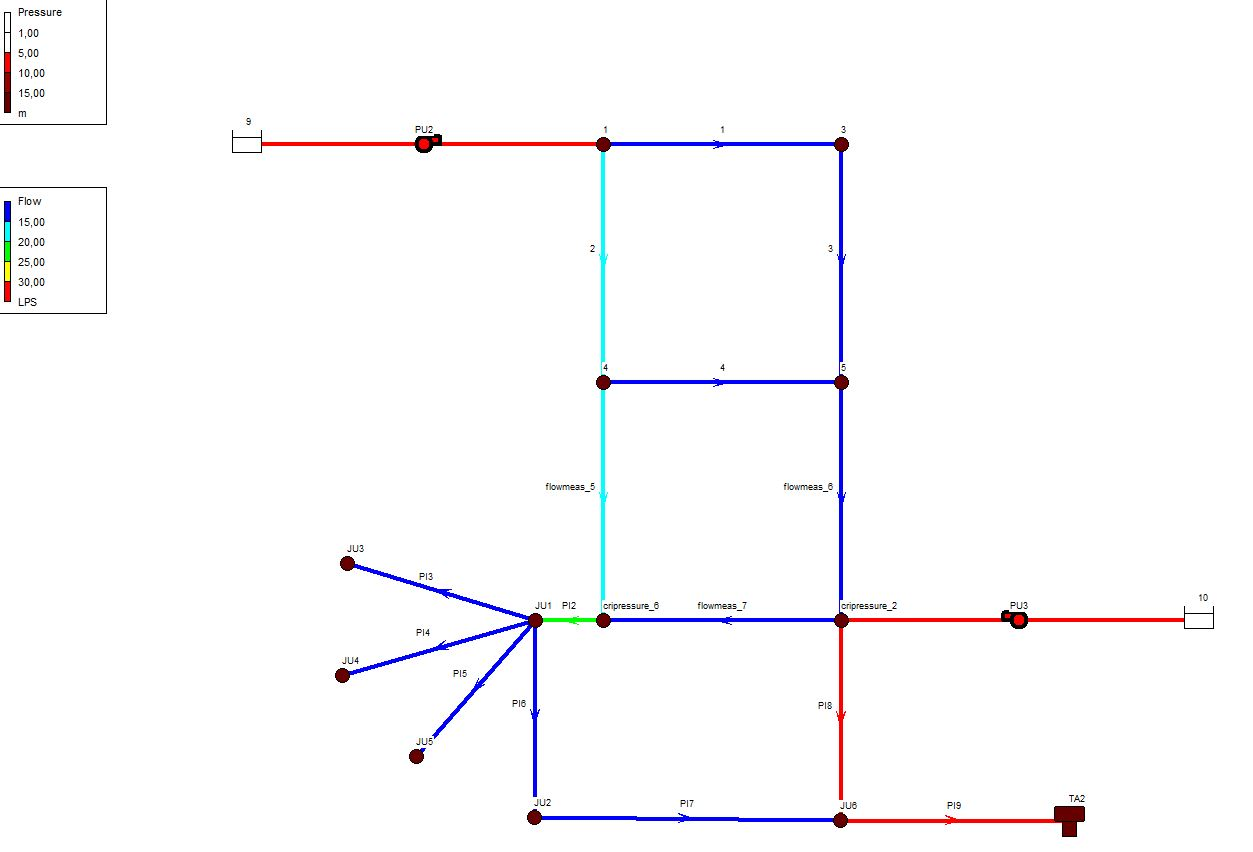
\includegraphics[width=0.65\textwidth]{discussion_files/example1}
%\begin{tikzpicture}[scale=0.6,transform shape]

\begin{scope} [rotate around={0:(12,5.5)}, shift={(0.8,0)}]
\draw[thick,transform shape] (12,5.5) circle (0.5);
\draw[thick,transform shape] (12.5,5.5) -- (12,6);
\draw[thick,transform shape] (12.5,5.5) node (v1) {} -- (12,5);
\end{scope}

%man-valve
\begin{scope} [rotate ={-90}]
\node(n1) at (-5.25,16) {};
\draw[thick,transform shape](n1.center) -- ($(n1)-(0.5,0)$) --
($(n1)-(0,1)$) -- ($(n1)-(0.5,1)$) --  (n1.center);

\end{scope}

\draw [thick](15,5.5) -- (13.3,5.5);
\node at (15.5,6.2) {\large PRV};
\draw [thick](16,5.5) -- (17.5,5.5);
\draw [fill=cyan] [thick](9.1,5.7) -- (9.1,5.1) -- (10.9,5.1) -- (10.9,5.7);
\draw  [thick](9.1,6.1) -- (9.1,5.1) -- (10.9,5.1) -- (10.9,6.1);
\draw [thick](12.3,5.5) -- (10.9,5.5);
\end{tikzpicture} 
\caption{Example network.}
\label{fig:example1}
\end{figure}
\vspace{-8mm}
The input data for identification consists of both the linear and non-linear inputs. Furthermore, feed-forward backpropagation model has been chosen for training. \figref{fig:inputs} shows the non-constant training and target data. 

\begin{figure}[H]
\centering
%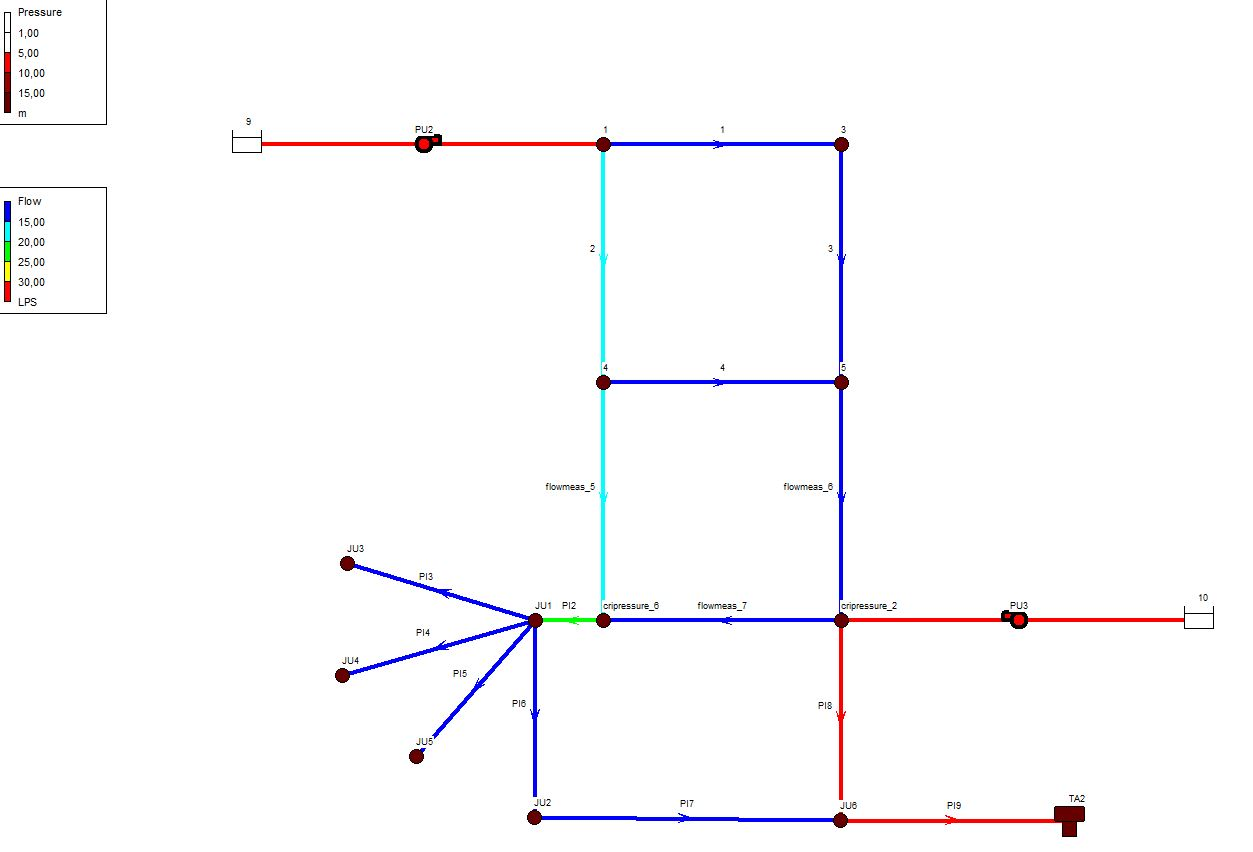
\includegraphics[width=1\textwidth]{discussion_files/example1}
% This file was created by matlab2tikz.
%
%The latest updates can be retrieved from
%  http://www.mathworks.com/matlabcentral/fileexchange/22022-matlab2tikz-matlab2tikz
%where you can also make suggestions and rate matlab2tikz.
%
\definecolor{mycolor1}{rgb}{0.00000,0.44700,0.74100}%
\definecolor{mycolor2}{rgb}{0.85000,0.32500,0.09800}%
%
\begin{tikzpicture}

\begin{axis}[%
width=1.931in,
height=1in,
at={(0.779in,2.636in)},
scale only axis,
xmin=0,
xmax=49,
xlabel style={font=\color{white!15!black}},
xlabel={Time [h]},
ymin=40.5,
ymax=40.8,
ylabel style={font=\color{white!15!black}},
ylabel={Pressure [m]},
axis background/.style={fill=white},
title style={font=\bfseries},
title={WT pressure}
]
\addplot[const plot, color=mycolor1, line width=1.2pt, forget plot] table[row sep=crcr] {%
0	40.5\\
1	40.56\\
2	40.55\\
3	40.57\\
4	40.56\\
5	40.6\\
6	40.67\\
7	40.73\\
8	40.72\\
9	40.73\\
10	40.73\\
11	40.76\\
12	40.8\\
13	40.8\\
14	40.78\\
15	40.8\\
16	40.79\\
17	40.8\\
18	40.8\\
19	40.8\\
20	40.78\\
21	40.8\\
22	40.79\\
23	40.8\\
24	40.8\\
25	40.8\\
26	40.78\\
27	40.8\\
28	40.79\\
29	40.8\\
30	40.8\\
31	40.8\\
32	40.78\\
33	40.8\\
34	40.79\\
35	40.8\\
36	40.8\\
37	40.8\\
38	40.78\\
39	40.8\\
40	40.79\\
41	40.8\\
42	40.8\\
43	40.8\\
44	40.78\\
45	40.8\\
46	40.79\\
47	40.8\\
};
\end{axis}

\begin{axis}[%
width=1.931in,
height=1in,
at={(3.348in,2.636in)},
scale only axis,
xmin=0,
xmax=49,
xlabel style={font=\color{white!15!black}},
xlabel={Time [h]},
ymin=40,
ymax=55,
ylabel style={font=\color{white!15!black}},
ylabel={Pressure [m]},
axis background/.style={fill=white},
title style={font=\bfseries},
title={Inlet pressures - Target}
]
\addplot[const plot, color=mycolor1, line width=1.2pt, forget plot] table[row sep=crcr] {%
0	44.87\\
1	42.18\\
2	42.93\\
3	42.45\\
4	43.64\\
5	45.4\\
6	44.97\\
7	42.31\\
8	43.05\\
9	42.58\\
10	43.75\\
11	45.5\\
12	51.68\\
13	42.36\\
14	43.1\\
15	42.63\\
16	43.79\\
17	52.42\\
18	51.68\\
19	42.36\\
20	43.1\\
21	42.63\\
22	43.79\\
23	51.68\\
24	51.68\\
25	42.36\\
26	43.1\\
27	42.63\\
28	43.79\\
29	52.42\\
30	51.68\\
31	42.36\\
32	43.1\\
33	42.63\\
34	43.79\\
35	52.42\\
36	51.68\\
37	42.36\\
38	43.1\\
39	42.63\\
40	43.79\\
41	52.42\\
42	51.68\\
43	42.36\\
44	43.1\\
45	42.63\\
46	43.79\\
47	51.68\\
};
\addplot[const plot, color=mycolor2, line width=1.2pt, forget plot] table[row sep=crcr] {%
0	43.81\\
1	41.22\\
2	41.89\\
3	41.46\\
4	42.57\\
5	44.37\\
6	43.93\\
7	41.36\\
8	42.02\\
9	41.6\\
10	42.69\\
11	44.48\\
12	51.51\\
13	41.41\\
14	42.07\\
15	41.66\\
16	42.74\\
17	52.33\\
18	51.51\\
19	41.41\\
20	42.07\\
21	41.66\\
22	42.74\\
23	51.51\\
24	51.51\\
25	41.41\\
26	42.07\\
27	41.66\\
28	42.74\\
29	52.33\\
30	51.51\\
31	41.41\\
32	42.07\\
33	41.66\\
34	42.74\\
35	51.51\\
36	51.51\\
37	41.41\\
38	42.07\\
39	41.66\\
40	42.74\\
41	51.51\\
42	41.41\\
43	42.07\\
44	41.66\\
45	42.74\\
46	51.51\\
47	51.51\\
};
\end{axis}

\begin{axis}[%
width=1.931in,
height=1in,
at={(0.779in,0.563in)},
scale only axis,
xmin=0,
xmax=49,
xlabel style={font=\color{white!15!black}},
xlabel={Time [h]},
ymin=10,
ymax=40,
ylabel style={font=\color{white!15!black}},
ylabel={Flows [LPS]},
axis background/.style={fill=white},
title style={font=\bfseries},
title={Inlet flows}
]
\addplot[const plot, color=mycolor1, line width=1.2pt, forget plot] table[row sep=crcr] {%
0	31.87\\
1	36.58\\
2	35.33\\
3	36.13\\
4	34.11\\
5	30.85\\
6	31.68\\
7	36.38\\
8	35.12\\
9	35.92\\
10	33.91\\
11	30.67\\
12	14.09\\
13	36.29\\
14	35.04\\
15	35.84\\
16	33.83\\
17	10.48\\
18	14.09\\
19	36.29\\
20	35.04\\
21	35.84\\
22	33.83\\
23	14.09\\
24	14.09\\
25	36.29\\
26	35.04\\
27	35.84\\
28	33.83\\
29	10.48\\
30	14.09\\
31	36.29\\
32	35.04\\
33	35.84\\
34	33.83\\
35	10.48\\
36	14.09\\
37	36.29\\
38	35.04\\
39	35.84\\
40	33.83\\
41	10.48\\
42	14.09\\
43	36.29\\
44	35.04\\
45	35.84\\
46	33.83\\
47	14.09\\
};
\addplot[const plot, color=mycolor2, line width=1.2pt, forget plot] table[row sep=crcr] {%
0	35.53\\
1	39.67\\
2	38.65\\
3	39.3\\
4	37.57\\
5	34.58\\
6	35.34\\
7	39.46\\
8	38.44\\
9	39.08\\
10	37.37\\
11	34.39\\
12	18.41\\
13	39.38\\
14	38.36\\
15	39\\
16	37.29\\
17	15.52\\
18	18.41\\
19	39.38\\
20	38.36\\
21	39\\
22	37.29\\
23	18.41\\
24	18.41\\
25	39.38\\
26	38.36\\
27	39\\
28	37.29\\
29	15.52\\
30	18.41\\
31	39.38\\
32	38.36\\
33	39\\
34	37.29\\
35	15.52\\
36	18.41\\
37	39.38\\
38	38.36\\
39	39\\
40	37.29\\
41	15.52\\
42	18.41\\
43	39.38\\
44	38.36\\
45	39\\
46	37.29\\
47	18.41\\
};
\end{axis}

\begin{axis}[%
width=1.931in,
height=1in,
at={(3.348in,0.563in)},
scale only axis,
xmin=0,
xmax=49,
xlabel style={font=\color{white!15!black}},
xlabel={Time [h]},
ymin=20,
ymax=100,
ylabel style={font=\color{white!15!black}},
ylabel={Flows [LPS]},
axis background/.style={fill=white},
title style={font=\bfseries},
title={Total demand}
]
\addplot[const plot, color=mycolor1, line width=1.2pt, forget plot] table[row sep=crcr] {%
0	32.5\\
1	84.5\\
2	65\\
3	78\\
4	52\\
5	26\\
6	32.5\\
7	84.5\\
8	65\\
9	78\\
10	52\\
11	26\\
12	32.5\\
13	84.5\\
14	65\\
15	78\\
16	52\\
17	26\\
18	32.5\\
19	84.5\\
20	65\\
21	78\\
22	52\\
23	26\\
24	26\\
25	32.5\\
26	84.5\\
27	65\\
28	78\\
29	52\\
30	26\\
31	32.5\\
32	84.5\\
33	65\\
34	78\\
35	52\\
36	26\\
37	32.5\\
38	84.5\\
39	65\\
40	78\\
41	52\\
42	26\\
43	32.5\\
44	84.5\\
45	65\\
46	78\\
47	52\\
};
\end{axis}
\end{tikzpicture}% 
\caption{Input data for training.}
\label{fig:inputs}
\end{figure}

The performance of the validation is shown in \figref{fig:performance}

\begin{figure}[H]
\centering
%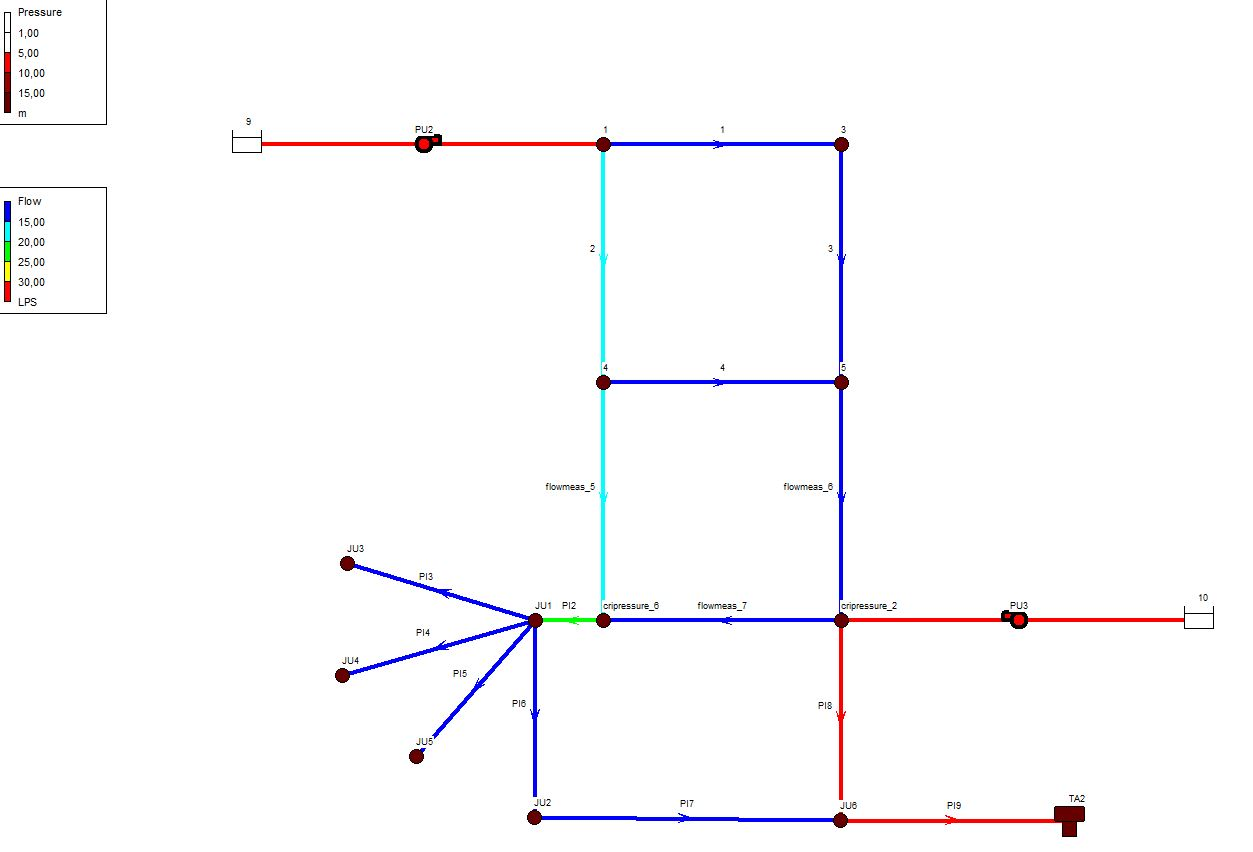
\includegraphics[width=1\textwidth]{discussion_files/example1}
% This file was created by matlab2tikz.
%
%The latest updates can be retrieved from
%  http://www.mathworks.com/matlabcentral/fileexchange/22022-matlab2tikz-matlab2tikz
%where you can also make suggestions and rate matlab2tikz.
%
\begin{tikzpicture}

\begin{axis}[%
width=2.521in,
height=1.866in,
at={(0.758in,0.481in)},
scale only axis,
unbounded coords=jump,
xmin=0,
xmax=55,
xlabel style={font=\bfseries\color{white!15!black}},
xlabel={55 Epochs},
ymode=log,
ymin=0.009,
ymax=110,
yminorticks=true,
ylabel style={font=\bfseries\color{white!15!black}},
ylabel={Mean Squared Error  (mse)},
axis background/.style={fill=white},
title style={font=\bfseries},
title={Best Validation Performance is 0.10993 at epoch 45},
axis x line*=bottom,
axis y line*=left,
legend style={legend cell align=left, align=left, draw=white!15!black}
]
\addplot [color=blue, line width=2.0pt]
  table[row sep=crcr]{%
0	54.5009116366302\\
1	25.2241191604978\\
2	5.11127033802924\\
3	3.28715468008978\\
4	2.37779684450367\\
5	2.19348705042348\\
6	2.1726917174479\\
7	2.16576732872671\\
8	2.1608551865329\\
9	2.14891323286878\\
10	2.14833137112214\\
11	2.1431825924294\\
12	2.14011221985651\\
13	2.13756186659183\\
14	2.13665194254738\\
15	2.13463793780153\\
16	2.13248048715957\\
17	2.13164414737313\\
18	2.12988523064693\\
19	2.12783241674969\\
20	2.12589323595964\\
21	2.12371913452639\\
22	2.1214200067441\\
23	2.11900840224138\\
24	2.11617214043734\\
25	2.11268216919153\\
26	2.11084486671493\\
27	2.1095898258682\\
28	2.10813504213467\\
29	2.10651798827363\\
30	2.10482920863136\\
31	2.10315722527777\\
32	2.10155692651044\\
33	2.10005339906147\\
34	2.0986576189817\\
35	2.09737529164666\\
36	2.0960749041136\\
37	2.08983712540624\\
38	2.08308428856932\\
39	2.08261633192981\\
40	2.08215235415385\\
41	2.08197143131414\\
42	2.08170894122243\\
43	2.08027174191013\\
44	2.07838900912088\\
45	2.07671367087435\\
46	2.07527739966795\\
47	2.0740544959996\\
48	2.07301830066111\\
49	2.07214498497574\\
50	2.07141180627356\\
51	2.07079672354041\\
52	2.07027910415953\\
53	2.06984054290616\\
54	2.06946528353388\\
55	2.06914019160894\\
};
\addlegendentry{\tiny Train}

\addplot [color=black!20!green, line width=2.0pt]
  table[row sep=crcr]{%
0	56.8004248212711\\
1	15.1657085291525\\
2	2.51311721353039\\
3	1.14944325686735\\
4	0.482202970655234\\
5	0.246480102565259\\
6	0.206969544649979\\
7	0.206746208059806\\
8	0.17237851916007\\
9	0.188397652354322\\
10	0.169256910601251\\
11	0.180510375234179\\
12	0.174978789462677\\
13	0.171554181011038\\
14	0.17333375481471\\
15	0.164957679337399\\
16	0.166201434104448\\
17	0.167587692902004\\
18	0.159729240192153\\
19	0.164035446892723\\
20	0.158932814243912\\
21	0.163486249086159\\
22	0.161748101952269\\
23	0.162975475791311\\
24	0.162968268436575\\
25	0.161970257156859\\
26	0.16543590551339\\
27	0.16311759554014\\
28	0.160492473821542\\
29	0.157754158367298\\
30	0.154919098384213\\
31	0.152170140052664\\
32	0.149662924382146\\
33	0.147457923267164\\
34	0.145558679755781\\
35	0.143948018991725\\
36	0.155894579828825\\
37	0.123907397795165\\
38	0.111438407870173\\
39	0.112196291927253\\
40	0.111719853384597\\
41	0.111187362207109\\
42	0.111113229818919\\
43	0.110638405769616\\
44	0.110007820316328\\
45	0.109934692050583\\
46	0.110337224306295\\
47	0.111004177559589\\
48	0.111777099537554\\
49	0.112560119701315\\
50	0.11330484830496\\
51	0.11399301959044\\
52	0.114623807543225\\
53	0.115205785215422\\
54	0.115752177035962\\
55	0.116278184592906\\
};
\addlegendentry{\tiny Validation}

\addplot [color=red, line width=2.0pt]
  table[row sep=crcr]{%
0	50.4449771281962\\
1	5.64485677553703\\
2	2.36338879551687\\
3	0.485864683014199\\
4	0.326248233652809\\
5	0.274425098520182\\
6	0.305333913067713\\
7	0.592232482497997\\
8	0.843068331904461\\
9	0.967077348148977\\
10	0.90039809683845\\
11	0.892901268559608\\
12	0.729285193940515\\
13	0.618990185319078\\
14	0.620099396274907\\
15	0.542774510937959\\
16	0.487513815504375\\
17	0.499349857269022\\
18	0.471167198119096\\
19	0.441725849816713\\
20	0.444742857859021\\
21	0.417388509763441\\
22	0.413422163984907\\
23	0.395831218037983\\
24	0.386372778482498\\
25	0.377309606195609\\
26	0.361117141093308\\
27	0.352303312113826\\
28	0.342997072260675\\
29	0.334425638967853\\
30	0.327339833670213\\
31	0.322060878877389\\
32	0.318532373622487\\
33	0.316535571971297\\
34	0.315830454568889\\
35	0.316192950146142\\
36	0.43516123901713\\
37	0.414779840608061\\
38	0.354133507520857\\
39	0.360236379228601\\
40	0.370759282550464\\
41	0.395597912132659\\
42	0.432831641839233\\
43	0.468774981628796\\
44	0.5002172543545\\
45	0.530026342813737\\
46	0.557861321545125\\
47	0.583191778763137\\
48	0.605811939125908\\
49	0.625822547761062\\
50	0.643513677402095\\
51	0.659248697586374\\
52	0.673386521106731\\
53	0.686241960077209\\
54	0.698072735508478\\
55	0.709080904815164\\
};
\addlegendentry{\tiny Test}

\addplot [color=black!52!green, dotted]
  table[row sep=crcr]{%
45	0.009\\
45	110\\
nan	nan\\
0	0.109934692050583\\
55	0.109934692050583\\
};
\addlegendentry{\tiny Best}

\addplot [color=black!52!green, line width=1.5pt, draw=none, mark size=8.0pt, mark=o, mark options={solid, black!52!green}, forget plot]
  table[row sep=crcr]{%
45	0.109934692050583\\
};
\addplot [color=black, dotted]
  table[row sep=crcr]{%
0	0.05\\
55	0.05\\
};
\addlegendentry{\tiny Goal}

\end{axis}
\end{tikzpicture}% 
\caption{Performance - MSE.}
\label{fig:performance}
\end{figure}

The validation goal is $0.05$ in Mean Squared Error (MSE). The training is stopped if either the goal is reached or the validation failure is more than 10 epochs. 

The training states are shown in \figref{fig:training}

\begin{figure}[H]
\centering
%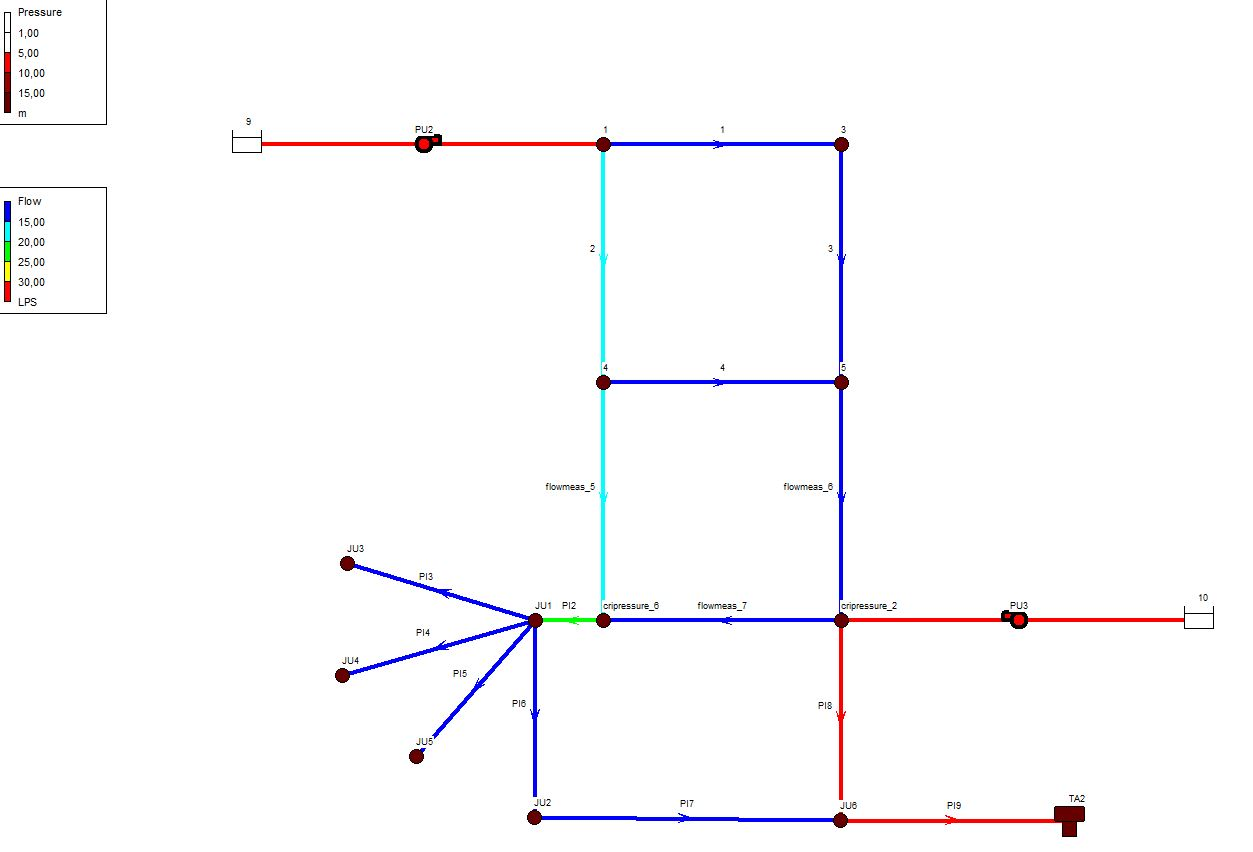
\includegraphics[width=1\textwidth]{discussion_files/example1}
% This file was created by matlab2tikz.
%
%The latest updates can be retrieved from
%  http://www.mathworks.com/matlabcentral/fileexchange/22022-matlab2tikz-matlab2tikz
%where you can also make suggestions and rate matlab2tikz.
%
\definecolor{mycolor1}{rgb}{0.00000,0.44700,0.74100}%
%
\begin{tikzpicture}

\begin{axis}[%
width=2.521in,
height=0.744in,
at={(0.758in,3.103in)},
scale only axis,
xmin=0,
xmax=55,
xtick={0,5,10,15,20,25,30,35,40,45,50,55},
xticklabels={\empty},
ymode=log,
ymin=0.01,
ymax=100,
yminorticks=true,
ylabel style={font=\color{white!15!black}},
ylabel={gradient},
axis background/.style={fill=white},
title style={font=\bfseries},
title={Gradient = 0.20823, at epoch 55}
]
\addplot [color=mycolor1, line width=2.0pt, forget plot]
  table[row sep=crcr]{%
0	86.8328678366811\\
1	45.2567871816596\\
2	21.5271608406747\\
3	13.2509551122308\\
4	4.26887566127795\\
5	0.640939747199987\\
6	0.340484816576075\\
7	0.429145230339779\\
8	1.16751349349841\\
9	0.32526930528258\\
10	0.830049177561905\\
11	0.0521923585066735\\
12	0.223968467201902\\
13	0.165066125897931\\
14	0.0479822766382217\\
15	0.286068099794094\\
16	0.163815296329578\\
17	0.0435904401098183\\
18	0.244988474876402\\
19	0.246512640194727\\
20	0.288395333901887\\
21	0.289625838835081\\
22	0.255622936360307\\
23	0.297337390569867\\
24	0.292444124442588\\
25	0.278229335963587\\
26	0.0243011909292663\\
27	0.0480836273526233\\
28	0.0690478372937888\\
29	0.0818272029421123\\
30	0.0786841779076867\\
31	0.0656551568702935\\
32	0.0517367306389594\\
33	0.0409734317090621\\
34	0.0335074949721925\\
35	0.0283063954658456\\
36	0.986009441876984\\
37	1.40418066892371\\
38	0.0559666669382676\\
39	0.244926783705835\\
40	0.392398489309648\\
41	0.727631884174076\\
42	1.06690091833268\\
43	1.12720319163119\\
44	1.03205802703222\\
45	0.931389052582064\\
46	0.837683106534759\\
47	0.74865609978875\\
48	0.661990991441159\\
49	0.577757764675057\\
50	0.497629227760707\\
51	0.423626757134112\\
52	0.35727632839899\\
53	0.299314065075387\\
54	0.249774124455642\\
55	0.208231977399724\\
};
\end{axis}

\begin{axis}[%
width=2.521in,
height=0.744in,
at={(0.758in,1.792in)},
scale only axis,
xmin=0,
xmax=55,
xtick={0,5,10,15,20,25,30,35,40,45,50,55},
xticklabels={\empty},
ymode=log,
ymin=0.0001,
ymax=0.01,
yminorticks=true,
ylabel style={font=\color{white!15!black}},
ylabel={mu},
axis background/.style={fill=white},
title style={font=\bfseries},
title={Mu = 0.001, at epoch 55}
]
\addplot [color=mycolor1, line width=2.0pt, forget plot]
  table[row sep=crcr]{%
0	0.001\\
1	0.001\\
2	0.001\\
3	0.001\\
4	0.001\\
5	0.001\\
6	0.001\\
7	0.001\\
8	0.001\\
9	0.001\\
10	0.001\\
11	0.01\\
12	0.001\\
13	0.001\\
14	0.01\\
15	0.001\\
16	0.001\\
17	0.01\\
18	0.001\\
19	0.001\\
20	0.001\\
21	0.001\\
22	0.001\\
23	0.001\\
24	0.001\\
25	0.001\\
26	0.01\\
27	0.01\\
28	0.01\\
29	0.01\\
30	0.01\\
31	0.01\\
32	0.01\\
33	0.01\\
34	0.01\\
35	0.01\\
36	0.001\\
37	0.0001\\
38	0.001\\
39	0.001\\
40	0.001\\
41	0.001\\
42	0.001\\
43	0.001\\
44	0.001\\
45	0.001\\
46	0.001\\
47	0.001\\
48	0.001\\
49	0.001\\
50	0.001\\
51	0.001\\
52	0.001\\
53	0.001\\
54	0.001\\
55	0.001\\
};
\end{axis}

\begin{axis}[%
width=2.521in,
height=0.744in,
at={(0.758in,0.481in)},
scale only axis,
xmin=0,
xmax=55,
xlabel style={font=\color{white!15!black}},
xlabel={55 Epochs},
ymin=0,
ymax=10,
ylabel style={font=\color{white!15!black}},
ylabel={val fail},
axis background/.style={fill=white},
title style={font=\bfseries},
title={Validation Checks = 10, at epoch 55}
]
\addplot [color=mycolor1, line width=1.0pt, draw=none, mark=diamond*, mark options={solid, fill=red, mycolor1}, forget plot]
  table[row sep=crcr]{%
0	0\\
1	0\\
2	0\\
3	0\\
4	0\\
5	0\\
6	0\\
7	0\\
8	0\\
9	1\\
10	0\\
11	1\\
12	2\\
13	3\\
14	4\\
15	0\\
16	1\\
17	2\\
18	0\\
19	1\\
20	0\\
21	1\\
22	2\\
23	3\\
24	4\\
25	5\\
26	6\\
27	7\\
28	8\\
29	0\\
30	0\\
31	0\\
32	0\\
33	0\\
34	0\\
35	0\\
36	1\\
37	0\\
38	0\\
39	1\\
40	2\\
41	0\\
42	0\\
43	0\\
44	0\\
45	0\\
46	1\\
47	2\\
48	3\\
49	4\\
50	5\\
51	6\\
52	7\\
53	8\\
54	9\\
55	10\\
};
\end{axis}
\end{tikzpicture}% 
\caption{Training states.}
\label{fig:training}
\end{figure}

For the training, Levenberg-Marquardt optimization was chosen to update weight and bias values. The validation of the output on the same data is shown in \figref{fig:output}

\begin{figure}[H]
\centering
%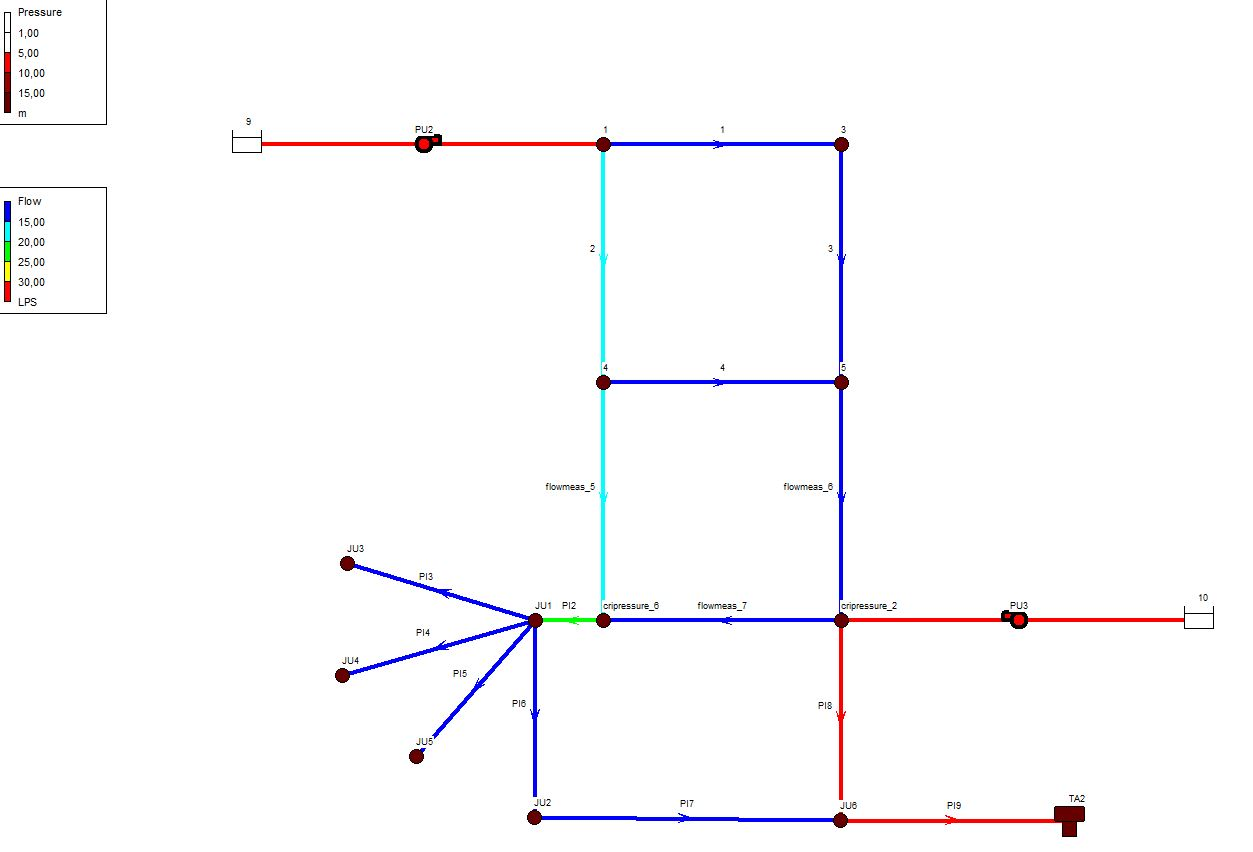
\includegraphics[width=1\textwidth]{discussion_files/example1}
% This file was created by matlab2tikz.
%
%The latest updates can be retrieved from
%  http://www.mathworks.com/matlabcentral/fileexchange/22022-matlab2tikz-matlab2tikz
%where you can also make suggestions and rate matlab2tikz.
%
\definecolor{mycolor1}{rgb}{0.00000,0.44700,0.74100}%
\definecolor{mycolor2}{rgb}{0.85000,0.32500,0.09800}%
%
\begin{tikzpicture}

\begin{axis}[%
width=2.1in,
height=1.8in,
at={(0.758in,0.481in)},
scale only axis,
xmin=0,
xmax=50,
xlabel style={font=\color{white!15!black}},
xlabel={Time [h]},
ymin=42,
ymax=55.5,
ylabel style={font=\color{white!15!black}},
ylabel={Pressure [m]},
axis background/.style={fill=white},
title style={font=\bfseries},
title={$\bar{p}_{K,1}$},
legend style={legend cell align=left, align=left, draw=white!15!black}
]
\addplot[const plot, color=mycolor1, line width=1.5pt] table[row sep=crcr] {%
0	44.9078603251918\\
1	42.1823541300428\\
2	42.8021974471182\\
3	42.4557944179844\\
4	43.6588844977126\\
5	45.4057421858801\\
6	44.8749507559613\\
7	42.2866938214854\\
8	43.2797359196819\\
9	42.6915326101042\\
10	43.6490727270893\\
11	44.7369653629794\\
12	51.9172618902386\\
13	42.2726365535345\\
14	42.9928792140575\\
15	42.6383018491128\\
16	43.6104251888554\\
17	52.6489276451398\\
18	51.9172618902386\\
19	42.2726365535345\\
20	42.9928792140575\\
21	42.6383018491128\\
22	43.6104251888554\\
23	51.5904218543352\\
24	51.5904218543352\\
25	42.6221049461825\\
26	42.9026793193479\\
27	42.5815145726614\\
28	43.8288222407025\\
29	52.3918775578125\\
30	51.5904218543352\\
31	42.6221049461825\\
32	42.9026793193479\\
33	42.5815145726614\\
34	43.8288222407025\\
35	52.3918775578125\\
36	51.5904218543352\\
37	42.6221049461825\\
38	42.9026793193479\\
39	42.5815145726614\\
40	43.8288222407025\\
41	52.3918775578125\\
42	51.5904218543352\\
43	42.6221049461825\\
44	42.9026793193479\\
45	42.5815145726614\\
46	43.8288222407025\\
47	51.749585263274\\
};
\addlegendentry{\tiny Model output}

\addplot[const plot, color=mycolor2, line width=1.5pt] table[row sep=crcr] {%
0	44.87\\
1	42.18\\
2	42.93\\
3	42.45\\
4	43.64\\
5	45.4\\
6	44.97\\
7	42.31\\
8	43.05\\
9	42.58\\
10	43.75\\
11	45.5\\
12	51.68\\
13	42.36\\
14	43.1\\
15	42.63\\
16	43.79\\
17	52.42\\
18	51.68\\
19	42.36\\
20	43.1\\
21	42.63\\
22	43.79\\
23	51.68\\
24	51.68\\
25	42.36\\
26	43.1\\
27	42.63\\
28	43.79\\
29	52.42\\
30	51.68\\
31	42.36\\
32	43.1\\
33	42.63\\
34	43.79\\
35	52.42\\
36	51.68\\
37	42.36\\
38	43.1\\
39	42.63\\
40	43.79\\
41	52.42\\
42	51.68\\
43	42.36\\
44	43.1\\
45	42.63\\
46	43.79\\
47	51.68\\
};
\addlegendentry{\tiny Training data}

\end{axis}

\begin{axis}[%
width=2.1in,
height=1.8in,
at={(3.327in,0.481in)},
scale only axis,
xmin=0,
xmax=50,
xlabel style={font=\color{white!15!black}},
xlabel={Time [h]},
ymin=40,
ymax=55.5,
ylabel style={font=\color{white!15!black}},
ylabel={Pressure [m]},
axis background/.style={fill=white},
title style={font=\bfseries},
title={$\bar{p}_{K,2}$},
legend style={legend cell align=left, align=left, draw=white!15!black}
]
\addplot[const plot, color=mycolor1, line width=1.5pt] table[row sep=crcr] {%
0	43.767861830952\\
1	41.1550878395116\\
2	41.4182885580612\\
3	41.4317548309122\\
4	42.5208090305292\\
5	44.0449578315806\\
6	43.9273381152115\\
7	40.1476000321916\\
8	42.4034031624744\\
9	41.1689404553921\\
10	42.4632046902127\\
11	42.6676855366913\\
12	51.3482316211594\\
13	41.4704539535611\\
14	41.8309680620566\\
15	42.2707284348765\\
16	43.0192709157775\\
17	52.2871672399964\\
18	51.3482316211594\\
19	41.4704539535611\\
20	41.8309680620566\\
21	42.2707284348765\\
22	43.0192709157775\\
23	49.5355598094426\\
24	49.5355598094426\\
25	41.3248935775008\\
26	42.0147583952019\\
27	41.5019405171386\\
28	44.7725363479986\\
29	51.8054581767913\\
30	49.5355598094426\\
31	41.3248935775008\\
32	42.0147583952019\\
33	41.5019405171386\\
34	44.7725363479986\\
35	51.8054581767913\\
36	49.5355598094426\\
37	41.3248935775008\\
38	42.0147583952019\\
39	41.5019405171386\\
40	44.7725363479986\\
41	51.8054581767913\\
42	49.5355598094426\\
43	41.3248935775008\\
44	42.0147583952019\\
45	41.5019405171386\\
46	44.7725363479986\\
47	51.4800719695692\\
};
\addlegendentry{\tiny Model output}

\addplot[const plot, color=mycolor2, line width=1.5pt] table[row sep=crcr] {%
0	43.81\\
1	41.22\\
2	41.89\\
3	41.46\\
4	42.57\\
5	44.37\\
6	43.93\\
7	41.36\\
8	42.02\\
9	41.6\\
10	42.69\\
11	44.48\\
12	51.51\\
13	41.41\\
14	42.07\\
15	41.66\\
16	42.74\\
17	52.33\\
18	51.51\\
19	41.41\\
20	42.07\\
21	41.66\\
22	42.74\\
23	51.51\\
24	51.51\\
25	41.41\\
26	42.07\\
27	41.66\\
28	42.74\\
29	52.33\\
30	51.51\\
31	41.41\\
32	42.07\\
33	41.66\\
34	42.74\\
35	51.51\\
36	51.51\\
37	41.41\\
38	42.07\\
39	41.66\\
40	42.74\\
41	51.51\\
42	41.41\\
43	42.07\\
44	41.66\\
45	42.74\\
46	51.51\\
47	51.51\\
};
\addlegendentry{\tiny Training data}

\end{axis}
\end{tikzpicture}% 
\caption{Outputs.}
\label{fig:output}
\end{figure}

The neurons used in this identification use Tan-Sigmoid transfer functions. Therefore the regression model with the corresponding weights and biases can be given 

\begin{equation}
\label{eq10}
y = B_2 + LW \cdot transig(B_1 + IW \cdot u).
\end{equation}

\emph{The documentation of theory and introduction of neural networks and system identification is in progress. First, I used this simple example to study and understand this approach. Some concerns and questions came up however, which we could discuss at the meeting.}

\subsection{Question reminders}
\emph{Q1}: Creating the input data

\emph{Q2}: Number of neurons

\emph{Q3}: RBF vs. MPL, training. 

\emph{Q4}: Validation on different data, check overfitting. 

\emph{Q5}: How to define linear/non-linear mixed model

\end{document}